% Capitolo 5 - Interfacce Grafiche ed Eventi
\chapter{Interfacce Grafiche ed Eventi}
\label{cap:interfacce_grafiche}

\section{Obiettivi di apprendimento}
Al termine di questo capitolo sarai in grado di:
\begin{itemize}
    \item Creare finestre grafiche utilizzando Swing
    \item Utilizzare i componenti base come JFrame, JPanel, JButton e JLabel
    \item Organizzare i componenti mediante Layout Manager
    \item Gestire eventi dell'utente con ActionListener
    \item Comprendere i concetti base di MouseEvent e KeyEvent
\end{itemize}

\section{Introduzione a Swing}

\textbf{Swing} è il framework principale per la creazione di interfacce grafiche (GUI) in Java. Fa parte delle Java Foundation Classes (JFC) e fornisce un insieme ricco di componenti per costruire applicazioni desktop.

\subsection{Caratteristiche principali}
\begin{itemize}
    \item \textbf{Portabilità}: le GUI Swing hanno lo stesso aspetto su tutte le piattaforme
    \item \textbf{Componenti leggeri}: i componenti Swing sono scritti completamente in Java
    \item \textbf{Ricchezza}: offre molti componenti predefiniti (pulsanti, tabelle, alberi, ecc.)
    \item \textbf{Personalizzabilità}: supporta Look and Feel diversi
\end{itemize}

\subsection{Gerarchia delle classi}
Tutti i componenti Swing ereditano da \texttt{JComponent}, che a sua volta eredita da \texttt{Component}. Le classi più comuni iniziano con la lettera "J" (JFrame, JButton, JPanel, ecc.). Questo meccanismo di ereditarietà è stato trattato nel \autoref{cap:classi_oggetti_ereditarieta}.

\section{Componenti principali}

\subsection{JFrame}
\texttt{JFrame} rappresenta la finestra principale dell'applicazione. È il contenitore di livello superiore.

\subsection{JPanel}
\texttt{JPanel} è un contenitore generico che può contenere altri componenti. Viene utilizzato per organizzare la GUI in sezioni logiche.

\subsection{JButton}
\texttt{JButton} è un pulsante cliccabile che può generare eventi.

\subsection{JLabel}
\texttt{JLabel} visualizza testo o immagini non modificabili dall'utente.

\subsection{Esempio integrato: Finestra con componenti base}

\begin{lstlisting}
import javax.swing.*;
import java.awt.*;
import java.awt.event.ActionEvent;
import java.awt.event.ActionListener;

public class FinestraBase extends JFrame {
    private JLabel etichetta;
    private JButton pulsante;
    private JPanel pannello;

    public FinestraBase() {
        // Configurazione della finestra (this e' un oggetto JFrame)
        this.setTitle("Applicazione Swing Base");
        this.setSize(400, 300);
        this.setDefaultCloseOperation(JFrame.EXIT_ON_CLOSE);
        this.setLocationRelativeTo(null); // Centra la finestra

        // Creazione componenti
        etichetta = new JLabel("Benvenuto nell'applicazione Swing!");
        etichetta.setFont(new Font("Arial", Font.BOLD, 16));
        etichetta.setHorizontalAlignment(SwingConstants.CENTER);

        pulsante = new JButton("Clicca qui");
        pulsante.setFont(new Font("Arial", Font.PLAIN, 14));

        // Aggiunta ActionListener al pulsante tramite pulsante.addActionListener()
        pulsante.addActionListener(new ActionListener() {
            @Override
            public void actionPerformed(ActionEvent e) {
                // Modifica il testo dell'etichetta quando il pulsante viene cliccato
                etichetta.setText("Hai cliccato il pulsante!");
            }
        });

        // Creazione pannello
        pannello = new JPanel();
        pannello.setLayout(new BorderLayout());
        pannello.add(etichetta, BorderLayout.CENTER);
        pannello.add(pulsante, BorderLayout.SOUTH);

        // Aggiunta pannello alla finestra tramite this.add()
        this.add(pannello);

        // Rende visibile la finestra tramite this.setVisible()
        this.setVisible(true);
    }

    public static void main(String[] args) {
        new FinestraBase();
    }
}
\end{lstlisting}

\section{Layout Manager}

I Layout Manager gestiscono automaticamente la disposizione dei componenti all'interno di un contenitore.

\subsection{BorderLayout}
Divide il contenitore in 5 aree: NORTH, SOUTH, EAST, WEST e CENTER.

\subsection{Esempio pratico BorderLayout}

\begin{lstlisting}
import javax.swing.*;
import java.awt.*;

public class EsempioBorderLayout extends JFrame {
    public EsempioBorderLayout() {
        // Configurazione della finestra (this e' un oggetto JFrame)
        this.setTitle("Esempio BorderLayout");
        this.setSize(500, 400);
        this.setDefaultCloseOperation(JFrame.EXIT_ON_CLOSE);

        // Il layout di default di JFrame e JPanel
        this.setLayout(new BorderLayout());

        // Creazione componenti per ogni area
        JButton btnNord = new JButton("NORTH - Barra del titolo");
        JButton btnSud = new JButton("SOUTH - Barra di stato");
        JButton btnEst = new JButton("EAST");
        JButton btnOvest = new JButton("WEST");
        JTextArea areaCentrale = new JTextArea("CENTER - Area principale");

        // Impostazione colori per visualizzare meglio le aree
        btnNord.setBackground(Color.CYAN);
        btnSud.setBackground(Color.YELLOW);
        btnEst.setBackground(Color.GREEN);
        btnOvest.setBackground(Color.ORANGE);
        areaCentrale.setBackground(Color.LIGHT_GRAY);

        // Aggiunta componenti nelle rispettive posizioni tramite this.add()
        this.add(btnNord, BorderLayout.NORTH);
        this.add(btnSud, BorderLayout.SOUTH);
        this.add(btnEst, BorderLayout.EAST);
        this.add(btnOvest, BorderLayout.WEST);
        this.add(new JScrollPane(areaCentrale), BorderLayout.CENTER);

        this.setVisible(true);
    }

    public static void main(String[] args) {
        new EsempioBorderLayout();
    }
}
\end{lstlisting}

\subsection{Altri Layout Manager comuni}

\begin{itemize}
    \item \textbf{FlowLayout}: dispone i componenti in sequenza, da sinistra a destra. Quando finisce lo spazio, va a capo.
    \item \textbf{GridLayout}: organizza i componenti in una griglia con righe e colonne di dimensioni uguali.
    \item \textbf{BoxLayout}: dispone i componenti in una singola riga o colonna.
    \item \textbf{GridBagLayout}: il più flessibile ma anche più complesso, permette disposizioni personalizzate.
\end{itemize}

\begin{lstlisting}
// Esempio FlowLayout
JPanel panelloFlow = new JPanel(new FlowLayout());
// Aggiunta componenti tramite panelloFlow.add()
panelloFlow.add(new JButton("Bottone 1"));
panelloFlow.add(new JButton("Bottone 2"));
panelloFlow.add(new JButton("Bottone 3"));

// Esempio GridLayout - griglia 2 righe x 3 colonne
JPanel panelloGrid = new JPanel(new GridLayout(2, 3));
for (int i = 1; i <= 6; i++) {
    // Aggiunta componenti tramite panelloGrid.add()
    panelloGrid.add(new JButton("Cella " + i));
}
\end{lstlisting}

\section{Gestione degli eventi con ActionListener}

Gli eventi permettono alle applicazioni di rispondere alle azioni dell'utente. \texttt{ActionListener} è un'interfaccia (vedi \autoref{cap:classi_oggetti_ereditarieta} per i concetti di interfaccia) usata per gestire eventi come click su pulsanti. Ogni componente che genera eventi fornisce metodi per registrare i listener, come il metodo \texttt{pulsante.addActionListener()} per i JButton.

\subsection{Esempio 1: Contatore di click}

\begin{lstlisting}
import javax.swing.*;
import java.awt.*;
import java.awt.event.ActionEvent;
import java.awt.event.ActionListener;

public class ContatoreClick extends JFrame {
    private JLabel lblContatore;
    private JButton btnIncrementa;
    private JButton btnReset;
    private int contatore;

    public ContatoreClick() {
        // Configurazione della finestra (this e' un oggetto JFrame)
        this.setTitle("Contatore di Click");
        this.setSize(350, 200);
        this.setDefaultCloseOperation(JFrame.EXIT_ON_CLOSE);
        this.setLayout(new BorderLayout());

        contatore = 0;

        // Etichetta per visualizzare il contatore
        lblContatore = new JLabel("Click: 0", SwingConstants.CENTER);
        lblContatore.setFont(new Font("Arial", Font.BOLD, 24));

        // Pannello per i pulsanti
        JPanel pannelloPulsanti = new JPanel(new FlowLayout());

        btnIncrementa = new JButton("Incrementa");
        btnReset = new JButton("Reset");

        // Aggiunta ActionListener al pulsante Incrementa tramite btnIncrementa.addActionListener()
        btnIncrementa.addActionListener(new ActionListener() {
            @Override
            public void actionPerformed(ActionEvent e) {
                contatore++;
                lblContatore.setText("Click: " + contatore);
            }
        });

        // Aggiunta ActionListener al pulsante Reset tramite btnReset.addActionListener()
        btnReset.addActionListener(new ActionListener() {
            @Override
            public void actionPerformed(ActionEvent e) {
                contatore = 0;
                lblContatore.setText("Click: " + contatore);
            }
        });

        pannelloPulsanti.add(btnIncrementa);
        pannelloPulsanti.add(btnReset);

        this.add(lblContatore, BorderLayout.CENTER);
        this.add(pannelloPulsanti, BorderLayout.SOUTH);

        this.setVisible(true);
    }

    public static void main(String[] args) {
        new ContatoreClick();
    }
}
\end{lstlisting}

\subsection{Esempio 2: Form di input semplice}

\begin{lstlisting}
import javax.swing.*;
import java.awt.*;
import java.awt.event.ActionEvent;
import java.awt.event.ActionListener;

public class FormInput extends JFrame {
    private JTextField txtNome;
    private JTextField txtCognome;
    private JButton btnSaluta;
    private JLabel lblRisultato;

    public FormInput() {
        // Configurazione della finestra (this e' un oggetto JFrame)
        this.setTitle("Form di Input");
        this.setSize(400, 250);
        this.setDefaultCloseOperation(JFrame.EXIT_ON_CLOSE);
        this.setLayout(new BorderLayout());

        // Pannello per i campi di input
        JPanel pannelloInput = new JPanel(new GridLayout(3, 2, 10, 10));
        pannelloInput.setBorder(BorderFactory.createEmptyBorder(10, 10, 10, 10));

        pannelloInput.add(new JLabel("Nome:"));
        txtNome = new JTextField(20);
        pannelloInput.add(txtNome);

        pannelloInput.add(new JLabel("Cognome:"));
        txtCognome = new JTextField(20);
        pannelloInput.add(txtCognome);

        btnSaluta = new JButton("Saluta");
        pannelloInput.add(new JLabel("")); // Cella vuota
        pannelloInput.add(btnSaluta);

        // Etichetta per il risultato
        lblRisultato = new JLabel("", SwingConstants.CENTER);
        lblRisultato.setFont(new Font("Arial", Font.BOLD, 16));

        // ActionListener per il pulsante tramite btnSaluta.addActionListener()
        btnSaluta.addActionListener(new ActionListener() {
            @Override
            public void actionPerformed(ActionEvent e) {
                String nome = txtNome.getText().trim();
                String cognome = txtCognome.getText().trim();

                if (nome.isEmpty() || cognome.isEmpty()) {
                    lblRisultato.setText("Inserisci nome e cognome!");
                    lblRisultato.setForeground(Color.RED);
                } else {
                    lblRisultato.setText("Ciao, " + nome + " " + cognome + "!");
                    lblRisultato.setForeground(Color.BLUE);
                }
            }
        });

        this.add(pannelloInput, BorderLayout.CENTER);
        this.add(lblRisultato, BorderLayout.SOUTH);

        this.setVisible(true);
    }

    public static void main(String[] args) {
        new FormInput();
    }
}
\end{lstlisting}

\begin{nota}
Per validare l'input dell'utente, utilizza il metodo dell'oggetto String \texttt{nome.trim()} per rimuovere spazi bianchi e il metodo dell'oggetto String \texttt{nome.isEmpty()} per verificare che il campo non sia vuoto.
\end{nota}

\section{Gestione avanzata degli eventi}

Oltre agli ActionListener, Swing supporta diversi tipi di eventi per una gestione più granulare dell'interazione utente. Comprendere il meccanismo degli eventi è fondamentale per creare applicazioni interattive e reattive.

\subsection{Tipi di eventi principali}

Java fornisce diverse classi di eventi per gestire le varie forme di interazione utente:

\begin{itemize}
    \item \textbf{ActionEvent}: generato da componenti come JButton, JMenuItem, JTextField (quando si preme Invio)
    \item \textbf{MouseEvent}: generato da azioni del mouse (click, movimento, pressione, rilascio)
    \item \textbf{KeyEvent}: generato da pressione/rilascio di tasti sulla tastiera
    \item \textbf{WindowEvent}: generato da operazioni sulle finestre (apertura, chiusura, ridimensionamento)
    \item \textbf{FocusEvent}: generato quando un componente acquisisce o perde il focus
    \item \textbf{ItemEvent}: generato da componenti di selezione come JCheckBox e JComboBox
\end{itemize}

\subsection{Meccanismo degli eventi: Listener e Adapter}

Il modello di gestione degli eventi in Java si basa sul \textbf{pattern Observer} (o Delegation Event Model), descritto in dettaglio nel \autoref{cap:lambda_expressions}. Funziona così:

\begin{enumerate}
    \item \textbf{Sorgente dell'evento}: il componente che genera l'evento (es. JButton)
    \item \textbf{Listener}: oggetto che "ascolta" l'evento implementando un'interfaccia specifica
    \item \textbf{Registrazione}: il listener viene registrato sulla sorgente tramite metodi dell'oggetto sorgente come \texttt{pulsante.addActionListener()}
    \item \textbf{Propagazione}: quando l'evento si verifica, il componente notifica tutti i listener registrati
\end{enumerate}

\begin{figure}[h]
\centering
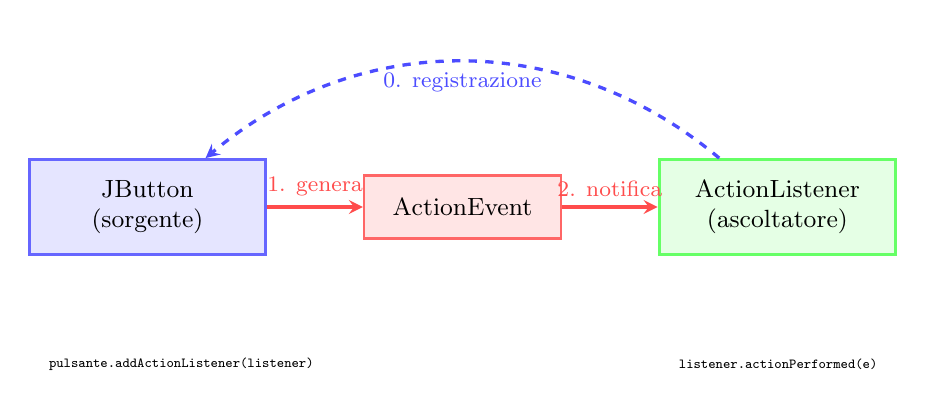
\begin{tikzpicture}[
    node distance=3cm,
    component/.style={
        rectangle,
        draw=blue!60,
        fill=blue!10,
        very thick,
        minimum width=3cm,
        minimum height=1.2cm,
        align=center,
        font=\small
    },
    event/.style={
        rectangle,
        draw=red!60,
        fill=red!10,
        thick,
        minimum width=2.5cm,
        minimum height=0.8cm,
        align=center,
        font=\small
    },
    arrow/.style={
        ->,
        >=stealth,
        very thick
    }
]

% Componente sorgente
\node[component] (button) at (0,0) {JButton\\(sorgente)};

% Evento
\node[event] (event) at (4,0) {ActionEvent};

% Listener
\node[component, fill=green!10, draw=green!60] (listener) at (8,0) {ActionListener\\(ascoltatore)};

% Frecce
\draw[arrow, red!70] (button) -- node[above, font=\footnotesize] {1. genera} (event);
\draw[arrow, red!70] (event) -- node[above, font=\footnotesize] {2. notifica} (listener);
\draw[arrow, blue!70, dashed, bend right=40] (listener) to node[below, font=\footnotesize] {0. registrazione} (button);

% Annotazioni
\node[font=\tiny, text width=2.5cm, align=left] at (0,-2) {
    \texttt{pulsante.addActionListener(listener)}
};

\node[font=\tiny, text width=2.5cm, align=left] at (8,-2) {
    \texttt{listener.actionPerformed(e)}
};

\end{tikzpicture}
\caption{Modello di gestione degli eventi: il listener si registra sul componente e viene notificato quando l'evento si verifica}
\label{fig:event_model}
\end{figure}

\subsubsection{Interfacce Listener vs Adapter}

Le interfacce listener (vedi \autoref{cap:classi_oggetti_ereditarieta} per i concetti di interfaccia) richiedono l'implementazione di tutti i metodi dichiarati. Gli \textbf{adapter} sono classi astratte di supporto che implementano tutte le interfacce con metodi vuoti, permettendo di sovrascrivere solo i metodi necessari:

\begin{center}
\begin{tabular}{|l|l|l|}
\hline
\textbf{Interfaccia} & \textbf{Adapter} & \textbf{Metodi} \\
\hline
\texttt{MouseListener} & \texttt{MouseAdapter} & 5 metodi \\
\hline
\texttt{KeyListener} & \texttt{KeyAdapter} & 3 metodi \\
\hline
\texttt{WindowListener} & \texttt{WindowAdapter} & 7 metodi \\
\hline
\texttt{FocusListener} & \texttt{FocusAdapter} & 2 metodi \\
\hline
\end{tabular}
\end{center}

\textbf{Esempio con Adapter:}

\begin{lstlisting}
// Senza adapter: dobbiamo implementare TUTTI i 5 metodi
// Registrazione tramite panel.addMouseListener()
panel.addMouseListener(new MouseListener() {
    public void mouseClicked(MouseEvent e) { /* logica */ }
    public void mousePressed(MouseEvent e) { }  // vuoto!
    public void mouseReleased(MouseEvent e) { } // vuoto!
    public void mouseEntered(MouseEvent e) { }  // vuoto!
    public void mouseExited(MouseEvent e) { }   // vuoto!
});

// Con adapter: sovrascriviamo SOLO quello che serve
// Registrazione tramite panel.addMouseListener()
panel.addMouseListener(new MouseAdapter() {
    @Override
    public void mouseClicked(MouseEvent e) {
        // Solo questo metodo viene sovrascritto
        // Uso del metodo e.getPoint() dell'oggetto MouseEvent
        System.out.println("Click a: " + e.getPoint());
    }
});
\end{lstlisting}

\subsection{Event Dispatch Thread (EDT)}

Tutti gli eventi GUI in Swing vengono gestiti da un thread speciale chiamato \textbf{Event Dispatch Thread} (EDT). È fondamentale rispettare queste regole:

\begin{enumerate}
    \item \textbf{Thread safety}: Tutti gli aggiornamenti ai componenti Swing devono avvenire nell'EDT
    \item \textbf{Non bloccare l'EDT}: Operazioni lunghe (lettura file, calcoli pesanti) devono essere eseguite in thread separati
    \item \textbf{Uso di SwingUtilities}: Per eseguire codice nell'EDT usa il metodo statico \texttt{SwingUtilities.invokeLater()}
\end{enumerate}

\begin{lstlisting}
// CORRETTO: Avvio dell'applicazione nell'EDT
public static void main(String[] args) {
    // Uso del metodo statico SwingUtilities.invokeLater()
    SwingUtilities.invokeLater(new Runnable() {
        @Override
        public void run() {
            new MiaApplicazione();
        }
    });
}

// CORRETTO: Operazione lunga in thread separato
// Registrazione tramite button.addActionListener()
// Nota: la sintassi "e ->" e' una lambda expression (vedi \autoref{cap:lambda_expressions})
button.addActionListener(e -> {
    new Thread(() -> {
        // Operazione lunga (es. download file)
        String risultato = operazioneLunga();

        // Aggiornamento GUI nell'EDT tramite SwingUtilities.invokeLater()
        SwingUtilities.invokeLater(() -> {
            // Uso del metodo label.setText() per aggiornare la GUI
            label.setText(risultato);
        });
    }).start();
});
\end{lstlisting}

\begin{attenzione}
\textbf{Errore comune}: Eseguire operazioni lunghe direttamente nell'event handler blocca l'interfaccia.

\begin{lstlisting}
// SBAGLIATO: blocca l'interfaccia!
// Registrazione tramite button.addActionListener()
// Nota: la sintassi "e ->" e' una lambda expression (vedi \autoref{cap:lambda_expressions})
button.addActionListener(e -> {
    for (int i = 0; i < 1000000000; i++) {
        // calcolo pesante... interfaccia bloccata!
    }
    // Uso del metodo label.setText() dopo calcolo lungo
    label.setText("Fatto!");
});
\end{lstlisting}

La finestra diventerà "non rispondente" durante il calcolo. Usa sempre thread separati per operazioni lunghe.
\end{attenzione}

\subsection{Eventi personalizzati}

Oltre agli eventi predefiniti, puoi creare eventi personalizzati estendendo \texttt{EventObject}:

\begin{lstlisting}
import java.util.EventObject;

// Evento personalizzato che estende EventObject
public class PunteggioEvent extends EventObject {
    private int punteggio;

    public PunteggioEvent(Object source, int punteggio) {
        super(source);
        this.punteggio = punteggio;
    }

    public int getPunteggio() {
        return punteggio;
    }
}

// Listener personalizzato (interfaccia)
public interface PunteggioListener {
    void punteggioModificato(PunteggioEvent e);
}

// Classe che genera eventi personalizzati
public class GestionePunteggio {
    private List<PunteggioListener> listeners = new ArrayList<>();
    private int punteggio = 0;

    // Metodo per registrare un listener tramite oggetto.addPunteggioListener()
    public void addPunteggioListener(PunteggioListener listener) {
        listeners.add(listener);
    }

    public void incrementaPunteggio(int valore) {
        punteggio += valore;
        notificaListeners();
    }

    // Notifica tutti i listener registrati
    private void notificaListeners() {
        PunteggioEvent evento = new PunteggioEvent(this, punteggio);
        for (PunteggioListener listener : listeners) {
            // Chiamata del metodo listener.punteggioModificato() su ogni listener
            listener.punteggioModificato(evento);
        }
    }
}
\end{lstlisting}

\subsection{Propagazione degli eventi}

Gli eventi in Swing seguono un meccanismo di \textbf{propagazione} dalla sorgente verso i container parent. Puoi interrompere la propagazione consumando l'evento:

\begin{lstlisting}
// Registrazione tramite panel.addMouseListener()
panel.addMouseListener(new MouseAdapter() {
    @Override
    public void mouseClicked(MouseEvent e) {
        System.out.println("Click sul pannello");
        // Uso del metodo e.consume() dell'oggetto MouseEvent per impedire la propagazione
        e.consume();
    }
});
\end{lstlisting}

\subsection{MouseListener}

\texttt{MouseListener} gestisce eventi del mouse come click, pressione, rilascio e passaggio del cursore.

\begin{lstlisting}
import javax.swing.*;
import java.awt.event.MouseEvent;
import java.awt.event.MouseListener;

public class EsempioMouse extends JFrame {
    private JLabel lblMessaggio;

    public EsempioMouse() {
        // Configurazione della finestra (this e' un oggetto JFrame)
        this.setTitle("Esempio MouseListener");
        this.setSize(400, 300);
        this.setDefaultCloseOperation(JFrame.EXIT_ON_CLOSE);

        lblMessaggio = new JLabel("Clicca ovunque nella finestra",
                                  SwingConstants.CENTER);

        // Aggiunta MouseListener alla label tramite lblMessaggio.addMouseListener()
        lblMessaggio.addMouseListener(new MouseListener() {
            @Override
            public void mouseClicked(MouseEvent e) {
                // Uso dei metodi e.getX() e e.getY() dell'oggetto MouseEvent
                lblMessaggio.setText("Click a: (" + e.getX() + ", " +
                                   e.getY() + ")");
            }

            @Override
            public void mousePressed(MouseEvent e) {
                lblMessaggio.setText("Mouse premuto");
            }

            @Override
            public void mouseReleased(MouseEvent e) {
                lblMessaggio.setText("Mouse rilasciato");
            }

            @Override
            public void mouseEntered(MouseEvent e) {
                lblMessaggio.setText("Mouse entrato");
            }

            @Override
            public void mouseExited(MouseEvent e) {
                lblMessaggio.setText("Mouse uscito");
            }
        });

        this.add(lblMessaggio);
        this.setVisible(true);
    }
}
\end{lstlisting}

\subsection{KeyListener}

\texttt{KeyListener} gestisce eventi della tastiera.

\begin{lstlisting}
import javax.swing.*;
import java.awt.event.KeyEvent;
import java.awt.event.KeyListener;

public class EsempioKey extends JFrame {
    private JTextField txtInput;
    private JLabel lblMessaggio;

    public EsempioKey() {
        // Configurazione della finestra (this e' un oggetto JFrame)
        this.setTitle("Esempio KeyListener");
        this.setSize(400, 200);
        this.setDefaultCloseOperation(JFrame.EXIT_ON_CLOSE);
        this.setLayout(new BorderLayout());

        txtInput = new JTextField();
        lblMessaggio = new JLabel("Digita qualcosa...",
                                  SwingConstants.CENTER);

        // Aggiunta KeyListener al campo di testo tramite txtInput.addKeyListener()
        txtInput.addKeyListener(new KeyListener() {
            @Override
            public void keyTyped(KeyEvent e) {
                // Chiamato quando un carattere viene digitato
            }

            @Override
            public void keyPressed(KeyEvent e) {
                // Uso del metodo statico KeyEvent.getKeyText() e del metodo e.getKeyCode()
                lblMessaggio.setText("Tasto premuto: " +
                                   KeyEvent.getKeyText(e.getKeyCode()));
            }

            @Override
            public void keyReleased(KeyEvent e) {
                // Uso del metodo statico KeyEvent.getKeyText() e del metodo e.getKeyCode()
                lblMessaggio.setText("Tasto rilasciato: " +
                                   KeyEvent.getKeyText(e.getKeyCode()));
            }
        });

        this.add(txtInput, BorderLayout.NORTH);
        this.add(lblMessaggio, BorderLayout.CENTER);

        this.setVisible(true);
    }
}
\end{lstlisting}

\begin{attenzione}
I listener con molti metodi (come \texttt{MouseListener}) possono essere semplificati usando le classi adapter (es. \texttt{MouseAdapter}), che forniscono implementazioni vuote di tutti i metodi, permettendoti di sovrascrivere solo quelli necessari.
\end{attenzione}

\section{Riepilogo}

In questo capitolo abbiamo esplorato i fondamenti delle interfacce grafiche in Java con Swing:

\begin{itemize}
    \item \textbf{Swing}: framework principale per GUI in Java
    \item \textbf{JFrame}: contenitore principale per finestre
    \item \textbf{JPanel, JButton, JLabel}: componenti base per costruire interfacce
    \item \textbf{Layout Manager}: sistemi per organizzare automaticamente i componenti (BorderLayout, FlowLayout, GridLayout)
    \item \textbf{ActionListener}: gestione eventi su pulsanti e componenti interattivi tramite metodi come \texttt{pulsante.addActionListener()}
    \item \textbf{MouseListener e KeyListener}: gestione eventi del mouse e della tastiera tramite metodi come \texttt{componente.addMouseListener()} e \texttt{componente.addKeyListener()}
    \item \textbf{Event Dispatch Thread}: thread speciale per gestire tutti gli eventi GUI
\end{itemize}

Le GUI Swing permettono di creare applicazioni desktop interattive e user-friendly, separando la logica di presentazione dal resto dell'applicazione.

\begin{nota}
Per applicazioni moderne, considera anche:
\begin{itemize}
    \item \textbf{JavaFX}: framework più moderno con supporto CSS e animazioni
    \item \textbf{Pattern MVC}: separa la logica della GUI dal modello dati (vedi \autoref{cap:model_view_controller})
\end{itemize}
\end{nota}
